\documentclass{ximera}
\title{Continuity and Discontinuity}
\begin{abstract}
\end{abstract}
\begin{document}
\maketitle
\begin{dialogue}
\item[Julia]What does it mean for a graph to be discontinuous? I don't get it!
\item[Dylan] I think it's like when there's a hole in the graph or something.
\item[James] Actually there are different kinds of discontinuities, but they can be hard to visualize so let's take a look!
\item[Altogether] LET'S DIVE IN!
\end{dialogue}
\section{Introduction}
\begin{question}
A function $f$ is said to be \textit{continuous at a point} $x = a$ if which three conditions are satisfied?
\begin{selectAll}
\choice[correct]{$f(a)$ is defined}
\choice{$f(a) \neq 0$}
\choice[correct]{$\displaystyle \lim_{x\to a} f(x)$ exists}
\choice[correct]{$\displaystyle \lim_{x\to a} f(x)=f(a)$}
\choice{$f(x)$ is linear}
\choice{$f(x) \neq f(a)$}
\end{selectAll}
\end{question}
\section{Example}
Take the function $f(x) = \dfrac{(1-x)^2}{1-x}$.

\begin{image}
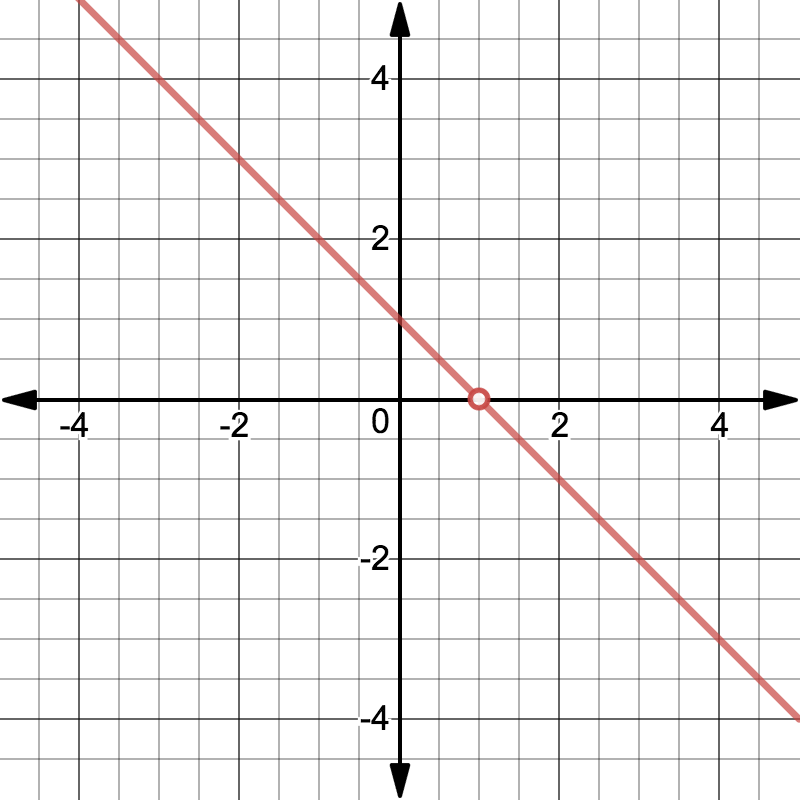
\includegraphics{continuity.png}
\end{image}

Through some simple elimination, we can easily see that this function is equivalent to $1-x$, where $x \neq 1$. Thus, there is one point on the original function we should pay close attention to: $x=1$.

Using the simple trick of squaring the denominator to create our numerator, we were able to easily pick a point where we will have a discontinuous function, without using a jump or infinite discontinuity. Jump discontinuities can easily be made using piecewise functions, and infinite discontinuities are often best made with rational functions, like fractions of polynomials! Don't worry if you haven't discussed these discontinuities yet; we'll see plenty in this lab!

\section{Problems}
\begin{question}
Consider the function $f(x)$:
\begin{image}
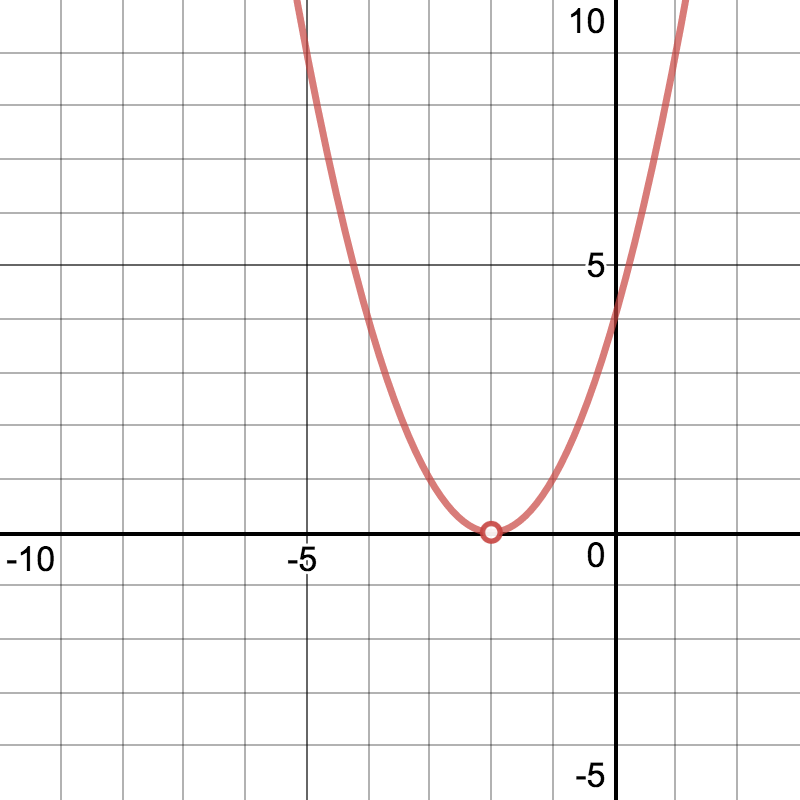
\includegraphics{continuity2}
\end{image}
Select all points which have a discontinuity.

\begin{selectAll}
\choice[correct]{$x=-2$}
\choice{$x=0$}
\choice{$x=-5$}
\choice{$x=5$}
\choice{$x=1$}
\choice{$x=-1$}
\end{selectAll}

What kind of discontinuity is present? Select all which apply.

\begin{selectAll}
\choice[correct]{Removable Discontinuity}
\choice{Jump Discontinuity}
\choice{Infinite Discontinuity}
\end{selectAll}

Using the format (*x-value*, *type of discontinuity*), indicate the x-values with their corresponding type of discontinuity. If multiple discontinuities exist, list them in ascending x-value order. Make sure to capitalize the type of discontinuity, and put commas following each ordered pair when necessary.

$\answer{(2, Removable)}$
\end{question}

\begin{question}
Consider the function $f(x)$:
\begin{image}
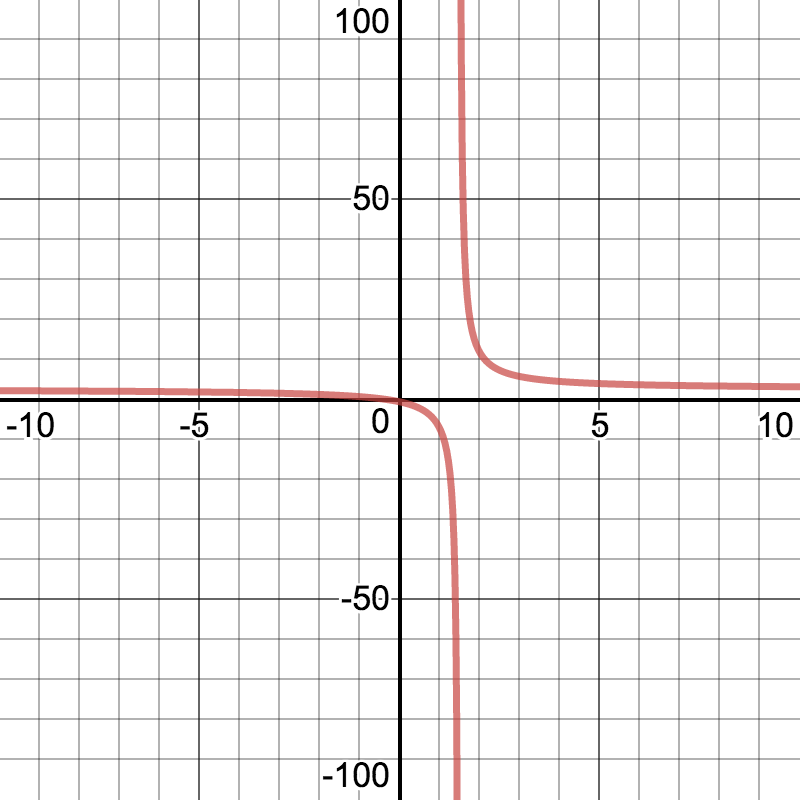
\includegraphics{continuity3}
\end{image}
Select all points which have a discontinuity.

\begin{selectAll}
\choice{$x=2$}
\choice{$x=0$}
\choice{$x=-2$}
\choice{$x=5$}
\choice[correct]{$x=1.5$}
\choice{$x=-1.5$}
\end{selectAll}

What kind of discontinuity is present? Select all which apply.

\begin{selectAll}
\choice{Removable Discontinuity}
\choice{Jump Discontinuity}
\choice[correct]{Infinite Discontinuity}
\end{selectAll}

Using the format (*x-value*, *type of discontinuity*), indicate the x-values with their corresponding type of discontinuity. If multiple discontinuities exist, list them in ascending x-value order. Make sure to capitalize the type of discontinuity, and put commas following each ordered pair when necessary.

$\answer{(2, Infinite)}$
\end{question}

\begin{question}
Consider the function $f(x)$:
\begin{image}
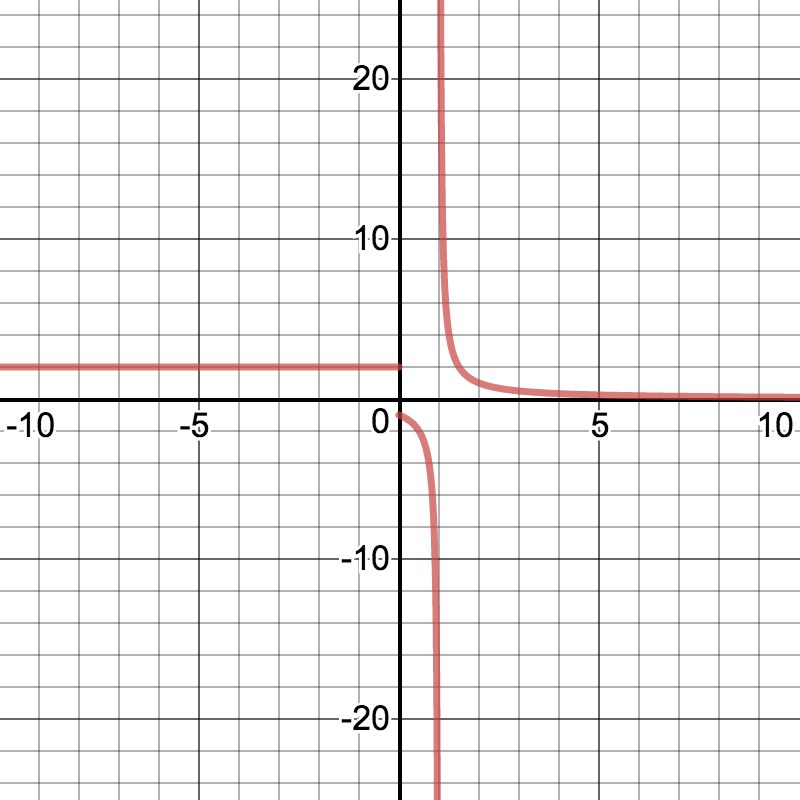
\includegraphics{continuity4}
\end{image}
Select all points which have a discontinuity.

\begin{selectAll}
\choice{$x=2$}
\choice[correct]{$x=0$}
\choice{$x=-5$}
\choice{$x=5$}
\choice[correct]{$x=1$}
\choice{$x=-1$}
\end{selectAll}

What kind of discontinuity is present? Select all which apply.

\begin{selectAll}
\choice[correct]{Removable Discontinuity}
\choice{Jump Discontinuity}
\choice[correct]{Infinite Discontinuity}
\end{selectAll}

Using the format (*x-value*, *type of discontinuity*), indicate the x-values with their corresponding type of discontinuity. If multiple discontinuities exist, list them in ascending x-value order. Make sure to capitalize the type of discontinuity, and put commas following each ordered pair when necessary.

$\answer{(0, Jump), (1, Infinite)}$
\end{question}

\begin{question}
Consider the function $f(x)$:
\begin{image}
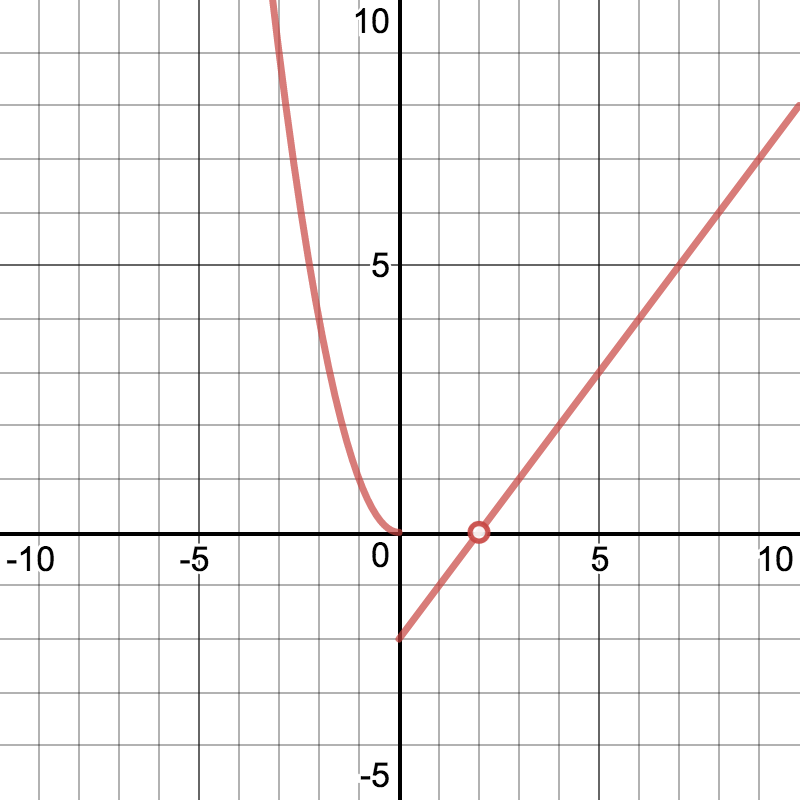
\includegraphics{continuity5}
\end{image}
Select all points which have a discontinuity.

\begin{selectAll}
\choice[correct]{$x=2$}
\choice[correct]{$x=0$}
\choice{$x=-2$}
\choice{$x=5$}
\choice{$x=1.5$}
\choice{$x=-1.5$}
\end{selectAll}

What kind of discontinuity is present? Select all which apply.

\begin{selectAll}
\choice[correct]{Removable Discontinuity}
\choice[correct]{Jump Discontinuity}
\choice{Infinite Discontinuity}
\end{selectAll}

Using the format (*x-value*, *type of discontinuity*), indicate the x-values with their corresponding type of discontinuity. If multiple discontinuities exist, list them in ascending x-value order. Make sure to capitalize the type of discontinuity, and put commas following each ordered pair when necessary.

$\answer{(0, Jump), (2, Removable)}$
\end{question}

\begin{question}
Consider the function $f(x)$:
\begin{image}
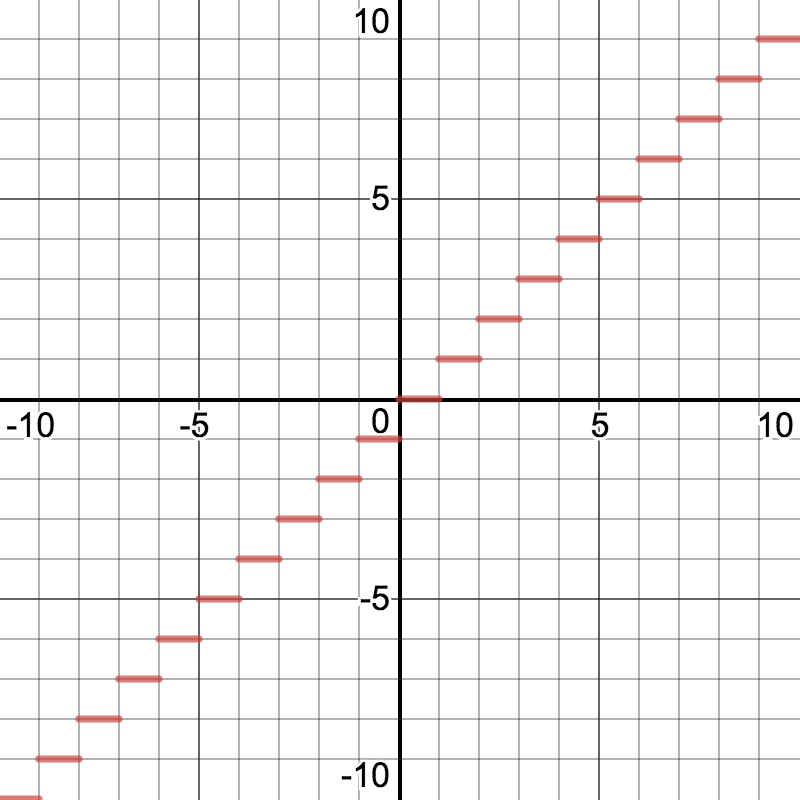
\includegraphics{continuity6}
\end{image}
Select all points which have a discontinuity.

\begin{selectAll}
\choice[correct]{$x=2$}
\choice[correct]{$x=0$}
\choice[correct]{$x=-2$}
\choice[correct]{$x=5$}
\choice{$x=1.5$}
\choice{$x=-1.5$}
\end{selectAll}

What kind of discontinuity is present? Select all which apply.

\begin{selectAll}
\choice{Removable Discontinuity}
\choice[correct]{Jump Discontinuity}
\choice{Infinite Discontinuity}
\end{selectAll}

\begin{hint}
Think of the different types of numbers - Rationals, Irrationals, Integers, Natural Numbers, Real Numbers, etc. If need be, look up what each of these are to refresh your memory.
\end{hint}
Indicate at what x-values the function is always discontinuous.

$\answer{Integers}$
\begin{feedback}
The function is discontinuous on both positive \textit{and} negative whole numbers. What are these numbers called?
\end{feedback}
\end{question}

\begin{dialogue}
\item[Julia] Whenever I see people talking about jump discontinuities, they always use piecewise functions. Do you think it's possible to make one without the function being piecewise?
\item[Dylan] If there's one thing that I've learned in math, it's that there are usually two ways to do anything! I'm not really sure how you would make something like that though...
\item[James] I know one function that would work!
\end{dialogue}

\begin{question}
\begin{hint}
James says the function has one value on the positives, the opposite of that on the negatives, and is undefined at 0.
\end{hint}
What function is James talking about?
$\answer{|x|/x}$
\end{question}

\begin{dialogue}
\item[Julia] Hey y'all, I was looking at our continuous graphs and noticed something.
\item[Dylan] What did you see? They all look like pretty normal functions to me.
\item[James] Yeah, I don't really know what you mean.
\item[Julia] Well, discontinuities mean there is a chunk of the graph where you can skip over a value, right? Like, we can jump right from 1 to 5, or have a hole where some value isn't attained.
\item[Dylan and James] Right. And?
\end{dialogue}

\begin{question}
\begin{hint}
Can we skip any of the values?
\end{hint}
What does Julia want to say about every value in a range $[f(a),f(b)]$ on a continuous graph?
\begin{multipleChoice}
\choice[correct]{Every value between $f(a)$ and $f(b)$ will be attained at some point on the interval $[a,b]$}
\choice{Only normal looking functions are continuous.}
\choice{No values that are not between $f(a)$ and $f(b)$ will be attained over the interval.}
\choice{No functional values are repeated over the interval.}
\end{multipleChoice}
\end{question}



\end{document}

